\documentclass{beamer}

\usepackage{fontspec}
\usepackage{xunicode}
\usepackage{xltxtra}
\usepackage{xecyr}
\usepackage{hyperref}
\usepackage{ragged2e}
\setmainfont[Mapping=tex-text]{DejaVu Serif}
\setsansfont[Mapping=tex-text]{DejaVu Sans}
\setmonofont[Mapping=tex-text]{DejaVu Sans Mono}
\usepackage{polyglossia}
\setdefaultlanguage{russian}
\usepackage{graphicx}
\usepackage{listings}

\renewcommand*{\inserttotalframenumber}{\pageref{lastframe}}

\lstdefinestyle{mycode}{
  belowcaptionskip=1\baselineskip,
  breaklines=true,
  xleftmargin=\parindent,
  showstringspaces=false,
  basicstyle=\footnotesize\ttfamily,
  keywordstyle=\bfseries,
  commentstyle=\itshape\color{gray!40!black},
  stringstyle=\color{red},
  numbers=left,
  numbersep=5pt,
  numberstyle=\tiny\color{gray},
}

\addtobeamertemplate{navigation symbols}{}{
    \usebeamerfont{footline}%
    \usebeamercolor[fg]{footline}%
    \hspace{1em}%
    {\small\color{black}{\insertframenumber/\inserttotalframenumber}}

}

\defbeamertemplate*{title page}{customized}[1][]{

  \begin{center}
  \usebeamerfont{institute}\insertinstitute\par
  \bigskip
  \usebeamerfont{title}\inserttitle\par
  \usebeamerfont{subtitle}\usebeamercolor[fg]{subtitle}\insertsubtitle\par
  \bigskip
  \color{black}{\usebeamerfont{author}\insertauthor}\par
  \bigskip
  {\scriptsize\usebeamerfont{date}\insertdate}\par
  \usebeamercolor[fg]{titlegraphic}\inserttitlegraphic
  \end{center}
}


%\let\otp\titlepage
%\renewcommand{\titlepage}{\otp\addtocounter{framenumber}{-1}}

\lstset{escapechar=@,style=mycode}
\setbeamerfont{frametitle}{size=\LARGE}

\title{Комплекс программ \\для автоматизации анализа популярности технологических 
областей в корпусе текстов русскоязычных электронных медиа}
%\subtitle{или как всё закодить в декабре, переписать в феврале и поседеть в апреле}
\author{{\small Антон Михайлович Алексеев, группа 532\\~\\ Руководитель~---~Т.В.~Тулупьева,~доц.,~доц.,~к.~пс.~н. \\ Рецензент~---~А.Е.~Пащенко,~~~н.~с.,~к.~т.~н.}}
\institute{Санкт-Петербургский государственный университет\\Математико-механический факультет\\ Кафедра информатики}
\date{4 июня 2014 г.}

\begin{document}

%\addtocounter{totalframenumber}{-1}

%1. Титульный слайд
% Генерируется автоматичсеки

{
\setbeamertemplate{navigation symbols}{} 
\frame{\titlepage}
}
%2. Структура доклада

\begin{frame}\frametitle{Структура доклада}
    \begin{enumerate}
        \item Введение
        \item Объект автоматизации
        \item Цель и задачи
        \item Данные и выбранный инструментарий
        \item Методы и комплекс программ
        \item Формальные признаки
        \item Результаты
    \end{enumerate}
\end{frame}

%%%3. Описание предметной области и формулировка проблемы, ее актуальность
\begin{frame}\frametitle{Введение}

\begin{itemize}
\item Маркетологические Интернет-исследования на основе текстов на ЕЯ
\item Объём данных слишком велик для <<ручного>> анализа
\item Богатый инструментарий для английского языка
\end{itemize}

\end{frame}

%4. Объект и предмет исследования ЛИБО объект автоматизации (зависит от типа дипломного проекта)
\begin{frame}
\textbf{Объект автоматизации}\\~\\
Подсчёт случаев совместных упоминаний технологических областей и наименований организаций в разное время во влиятельных СМИ\\~\\
\textbf{Цель}\\~\\
Разработка комплекса программ, способного установить взаимосвязь упоминаний технологических областей и наименований
организаций в блогах или новостях на русском языке на основе корпуса текстов электронных медиа 
\end{frame}

\begin{frame}\frametitle{Задачи}

\begin{enumerate}
    \item Cбор тестовых данных
    \item Модуль, выделяющий из текста наименования организаций
    \item Модуль, выделяющий из текста технологические области
    \item Модуль, осуществляющий построение табличных отчётов по результатам двух последних задач
    \item Модуль, осуществляющий визуализацию отчётов в виде графиков
\end{enumerate}
\end{frame}

\begin{frame}\frametitle{Схема обработки данных}
\begin{figure}[ht]
\begin{center}
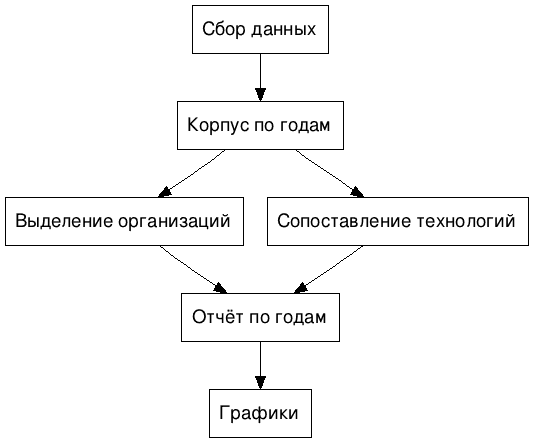
\includegraphics[height=3in]{pipeline.png}
\end{center}
\end{figure}
\end{frame}

%6. (Подходы к решению, решения, использованный инструментарий)
\begin{frame}\frametitle{Источники данных}

\begin{itemize}
    \item CrunchBase
    \item Habrahabr.ru
    \item Lenta.ru: <<Наука и техника>>
    \item Русскоязычная и англоязычная версии Википедии
\end{itemize}

\end{frame}

\begin{frame}\frametitle{Структура Википедии [1]}
Помимо статей, текстовых ссылок и заголовков, пользователями Википедии поддерживается <<дерево категорий>>

\begin{figure}[ht]
\begin{center}
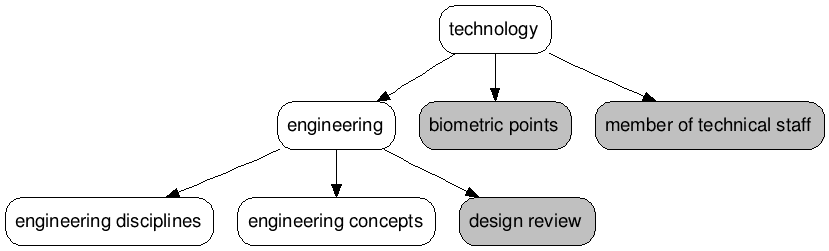
\includegraphics[width=4.5in]{chart_categories.png}
\end{center}
\end{figure}

\end{frame}
\begin{frame}\frametitle{Структура Википедии [2]}

\begin{figure}[ht]
\begin{center}
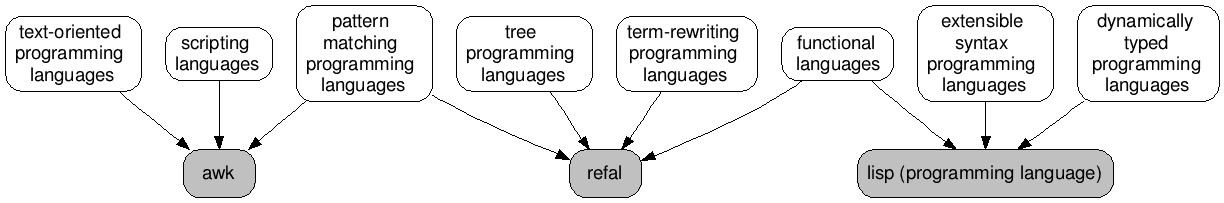
\includegraphics[width=4.5in]{chart_languages.png}
\end{center}
\end{figure}
\end{frame}


%7. Программный комплекс/программа: состав, архитектура, диаграммы
%классов, структура БД, фуекциональность, результаты работы и пр.
\begin{frame}\frametitle{Извлечение наименований организаций}
\begin{enumerate}
\item Токенизация
\item Стемминг
\item Поиск подстрок из сформированного списка нормализованных наименований организаций
\end{enumerate}
Стемминг --- один из видов нормализации токенов; как правило, под этим термином понимают эвристический процесс «отрезания» окончаний слов
\end{frame}

\begin{frame}\frametitle{Извлечение технологических областей~[1]}
Первый этап --- предобработка
        \begin{enumerate}
		\item Токенизация
		\item Фильтрация по списку стоп-слов
		\item Фильтрация по списку нормализованных слов, встречавшихся в текстах ссылок и заголовков Википедии
        \end{enumerate}

\end{frame}

%\begin{frame}\frametitle{Извлечение технологических областей~[2]}
%\begin{enumerate}
%         \setcounter{enumi}{1}
%        \item Поиск технологических областей
%        \begin{enumerate} %
%		\item Поиск в тексте заголовков русскоязычной Википедии с помощью инвертированного индекса Lucene
%		\item Переход к англоязычным версиям найденных статей
%		\item ~<<Восхождение>> по BFS-дереву категории \textbf{Technology} в графе категорий англоязычной версии Википедии
%		 \item Запоминание всех посещённых вершин графа как технологических областей
%       \end{enumerate}
%\end{enumerate}
%\end{frame}

\begin{frame}\frametitle{Извлечение технологических областей~[2]}

\begin{figure}[ht]
\begin{center}
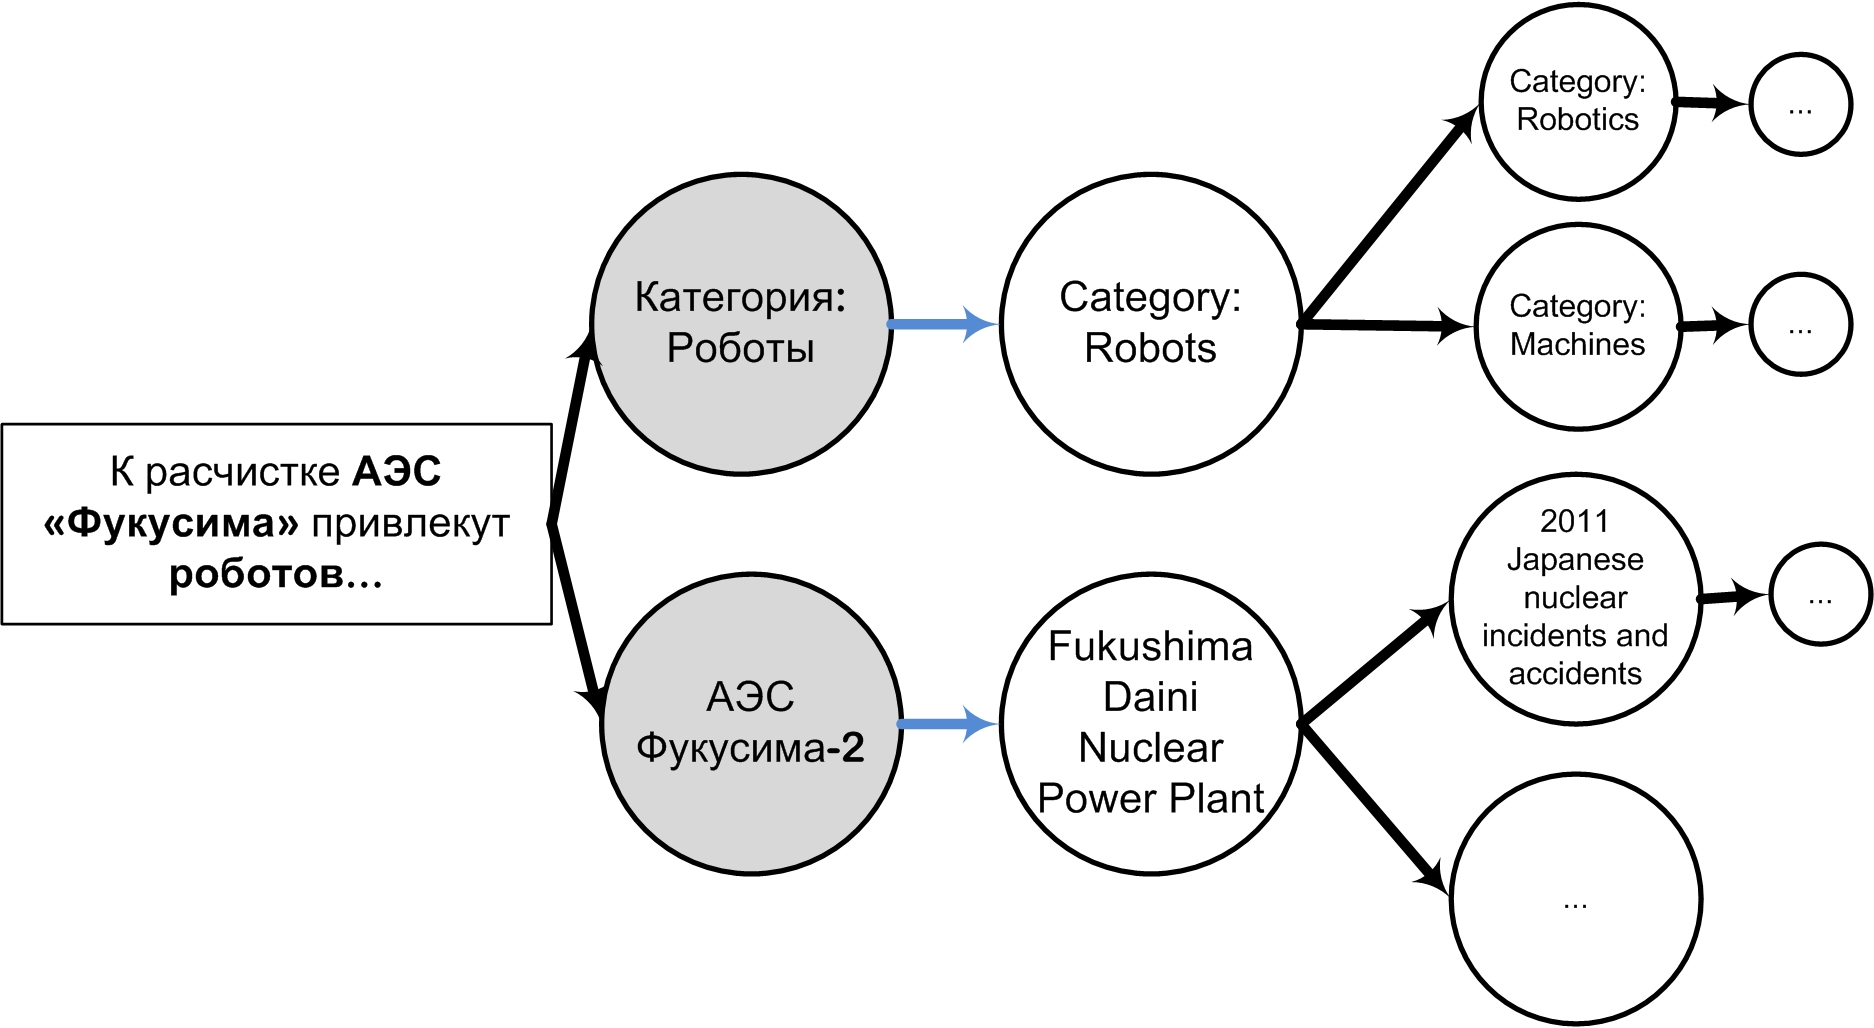
\includegraphics[width=4.5in]{Process.png}
\end{center}
\end{figure}

\end{frame}

\begin{frame}\frametitle{Примеры графиков [1]}
\begin{figure}[ht]
\begin{center}
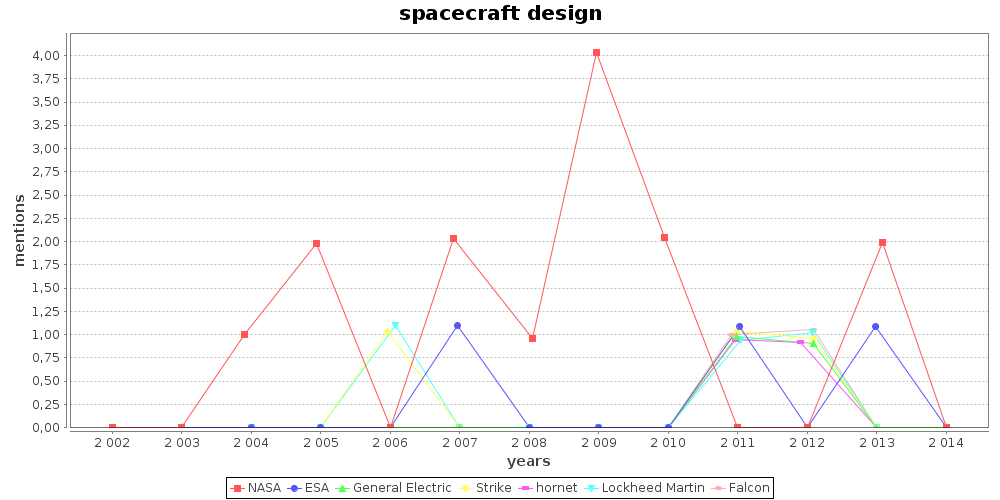
\includegraphics[width=4.5in]{space.png}
\end{center}
\end{figure}
\end{frame}

\begin{frame}\frametitle{Примеры графиков [2]}
\begin{figure}[ht]
\begin{center}
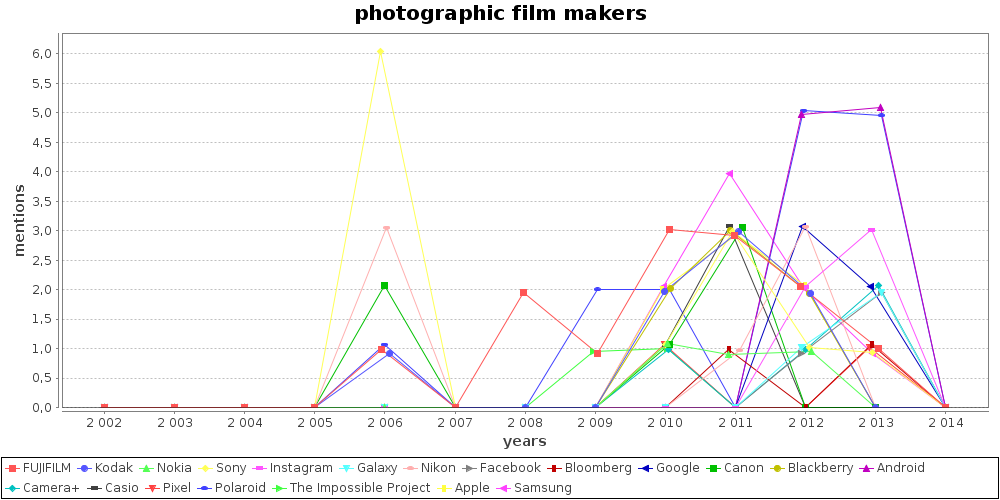
\includegraphics[width=4.5in]{film.png}
\end{center}
\end{figure}
\end{frame}

\begin{frame}\frametitle{Пример графического интерфейса}
\begin{figure}[ht]
\begin{center}
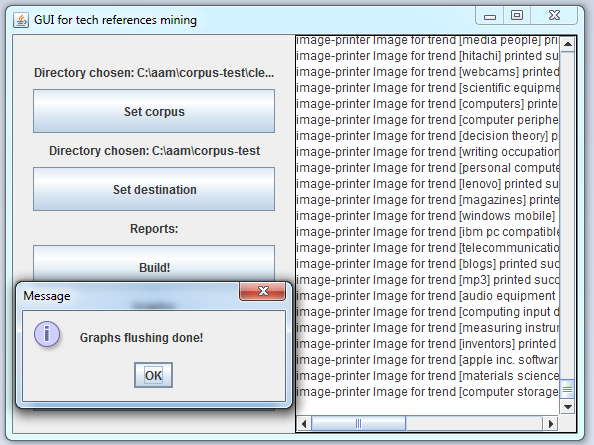
\includegraphics[height=2.5in]{gui.png}
\end{center}
\end{figure}
\end{frame}


\begin{frame}\frametitle{Использованный инструментарий}

\begin{itemize}
    \item Scala
    \item Java
    \item Python
    \item WikiXMLJ
    \item slf4j + logback
    \item Apache Commons
    \item Apache Lucene
    \item Apache Maven
\end{itemize}

\end{frame}


\begin{frame}\frametitle{Формальные признаки}
\begin{itemize}
    \item Подход представлен на <<СПИСОК-2014>>
    \item Доклад принят на <<НСМВ-2014>>
    \item Более 5000 строк программного кода на Scala, Java и Python и XML-разметки
\end{itemize}
\end{frame}

%10. Повтор титульного слайда

{
\setbeamertemplate{navigation symbols}{} 
\frame{\titlepage\label{lastframe}}
}

{

\setbeamertemplate{navigation symbols}{} 
\begin{frame}\frametitle{Выбор значимых технологических областей}
$$\textrm{keyphraseness}=\frac{\textrm{Freq}_{link}}{\textrm{Freq}_{body}}$$
\end{frame}
}
\end{document}
